\documentclass{scrreprt}

%Packages, die für die deutsch Sprache erforderlich sind
\usepackage[utf8]{inputenc}
\usepackage[T1]{fontenc}
\usepackage{lmodern}
\usepackage{ngerman}

%Packages für Graphik
\usepackage{graphicx}
\graphicspath{{Abbildungen/}}

%Package, damit Bibtex-URL klappt
\usepackage{url}

\begin{document}
%%%%% BEGINN TITELSEITE %%%%%
\begin{titlepage}

% Oberer Teil der Titelseite:
\begin{minipage}{0.4\textwidth}
	\begin{flushleft}
		
\includegraphics[height=1.5cm]{TU_Logo}
	\end{flushleft}
\end{minipage}
\hfill
\begin{minipage}{0.4\textwidth}
	\begin{flushright}
		
\includegraphics[height=1.5cm]{MPM_Logo}%TODO: Logo in HQ
	\end{flushright}
\end{minipage}

\begin{center}    
\textbf{\LARGE Technische Universität Berlin}\\
\large{Institut für Konstruktion, Mikro- und Medizintechnik}\\
\large{Fachgebiet Methoden der Produktentwicklung und Mechatronik}\\
\large{\textsc{Prof. Dr.-Ing. Dietmar Göhlich}}\\
\vfill

% Title
\huge{\textbf{Vergleich von Ladesystemen und Speichertechnologien für batteriebetriebene Stadtbusse}}\\
\rule{\linewidth}{1pt}
\large{Zur Erlangung des akademischen Grades Bachelor of Science}\\
\large{Im Studiengang Informationstechnik im Maschinenwesen}\\
\vfill

%Autor
\large{\textsc{Ludger Heide}}\\
\large{Matrikelnummer 338641}\\
\vfill

\large{Betreuerin: \textsc{M.Sc. Tu-Anh Ly}}\\
\vfill

\large{\today}
\end{center}
\end{titlepage}
%%%%% ENDE TITELSEITE %%%%%

\pagenumbering{Roman}
\chapter*{Abstract}
\addcontentsline{toc}{chapter}{Abstract}
\section*{English}
\section*{Deutsch}

\chapter*{Aufgabenstellung}
\addcontentsline{toc}{chapter}{Aufgabenstellung}

\chapter*{Eidesstattliche Erklärung}
\addcontentsline{toc}{chapter}{Eidesstattliche Erklärung}
Ich, Ludger Heide, versichere hiermit, dass ich meine Bachelorarbeit mit dem Thema
\begin{quote}
	\emph{Vergleich von Ladesystemen und Speichertechnologien für batteriebetriebene Stadtbusse}
\end{quote}
selbstständig verfasst und keine anderen als die angegebenen Quellen und Hilfsmittel benutzt habe, wobei ich alle wörtlichen und sinngemäßen Zitate als solche gekennzeichnet habe. Die Arbeit wurde bisher keiner anderen Prüfungsbehörde vorgelegt und auch nicht veröffentlicht.\\[6ex]
Berlin, \today\\
\newline
\rule{4cm}{0.5pt}\\
\textsc{Ludger Heide} 

\tableofcontents

\listoffigures
\addcontentsline{toc}{chapter}{Abbildungsverzeichnis}

\listoftables
\addcontentsline{toc}{chapter}{Tabellenverzeichnis}
\newpage

%%%%% BEGINN INHALT %%%%%
\pagenumbering{arabic}

\chapter{Einleitung}
\section{Kontext} %Namen ändern!
\subsection{Geschichte}
\subsection{Aktueller Stand}
\section{Problem} %TODO Namen ändern
\subsection{Ziel} %TODO: Nur im Text erwähnen?
\section{Methodik} %(Kurz))
\chapter{Ladesysteme} %Zewitens
\section{Bewertungskriterien} %TODO: Subsections
% Mit welcher Methode ausgewählt?
\section{Betrachtete Systeme} %TODO: Subsections
\section{Vergleichstabelle}
\chapter{Speichertechnologien} %Zuerst
Nach den Ladesystemen werden in diesem Kapitel nun die Energiespeicher für Stadtbusse betrachtet. Wie im vorigen Kapitel werden zunächst die Bewertungskriterien und die betrachteten Technologien erläutert. In Tabelle \ref{vergleichstabelle_speichertechnologien} auf Seite \pageref{vergleichstabelle_speichertechnologien} werden die Werte aufgelistet.\\
Im Gegensatz zu den Ladesystemen ist die Produktvielfalt der Speichertechnologien nahezu unbegrenzt. Von daher werden hier keine konkreten Produkte verglichen, sondern es wurde versucht, die jeweils für den aktuellen Stand der Speichertechnologie relevanten Kenndaten zu finden.
\section{Bewertungskriterien} %TODO: Subsections
\section{Betrachtete Technologien}
Im folgenden Abschnitt werden die Grundlagen und die Einsatzgeschichten der verschiedenen Speichertechnologien kurz erläutert. Die Technologien sind nach dem genutzten physikalischen Effekt aufgeteilt \cite{Sterner:2014}[S. 35f].
\subsection{Mechanisch – Schwungradspeicher} %TODO: Quellen, warum endete die Gyrobuserprobung
In Bussen kann mechanische Energie mit einem Schwungrad gespeichert werden\footnote{Es gibt auch Prototypen von Pressluftspeichern in kleineren Fahrzeugen, in Bussen werden sie jedoch nur als Teil eines Hybridantriebs eingesetzt und hier nicht weiter betrachtet \cite{Sebastian-Naumann:2014}[S. 14].}, das die elektrische Energie in der Rotation des Schwungrades speichert. Die Energieübertragung erfolgt durch eine elektrische Motor- und Generatoreinheit. Moderne Schwungräder werden aus gewickelten Karbonfasern hergestellt und in Vakuumgehäusen magnetisch gelagert, sie erreichen hohe Drehzahlen und geringe Reibungsverluste \cite{993788}. Im Falle eines berstenden Schwungrades muss das Gehäuse die gesamte Energie innerhalb von Sekundenbruchteilen aufnehmen, ohne selbst zu bersten. Dies erfordert sehr schwere Gehäuse, die die spezifische Energie und Leistung eines tatsächlichen Systems stark reduzieren. Der Schwungradspeicher wurde in den fünfziger Jahren im Gyrobus im schweizerischen Yverdon auf einer acht Kilometer langen Linie erprobt. Die Strecke wurde erfolgreich zurückgelegt, die damalige Technologie war jedoch sehr wartungsaufwändig. Aktuell wird der Schwungradspeicher nur als Teil eines hybriden Antriebsstrangs eingesetzt.
\subsection{Elektrisch – Kondensator} %TODO: Quellen
Der Kondensator ist ein rein elektrischer Energiespeicher. Im klassischen Plattenkondensator werden zwei durch einen festes Dielektrikum getrennte Platten elektrisch aufgeladen, die Ladung kann später in Strom umgewandelt werden. Kondensatoren haben eine hohe spezifische Leistung, aber eine sehr geringe spezifische Energie. In Bussen werden sogenannte Superkondensatoren verwendet, die statt eines festen Dielektrikums ein Elektrolyt (meist eine Salz-Wasser-Lösung) verwenden. Die gelösten Ionen werden von der geladenen Platte angezogen, können sie jedoch aufgrund der umgebenden Ionenschicht nicht erreichen. Da der Abstand zwischen Platte un Ionen extrem klein ist, entsteht eine sehr hohe elektrische Kapazität. Eine weitere Kapazitätssteigerung wird durch die Einlagerung von einigen Elektronen des Elektrolyts in den Leiterplatten erreicht (siehe Abb. \ref{abb_doppelschicht}). \cite{Sterner:2014}[S. 167f]\\
\begin{figure}\centering
	 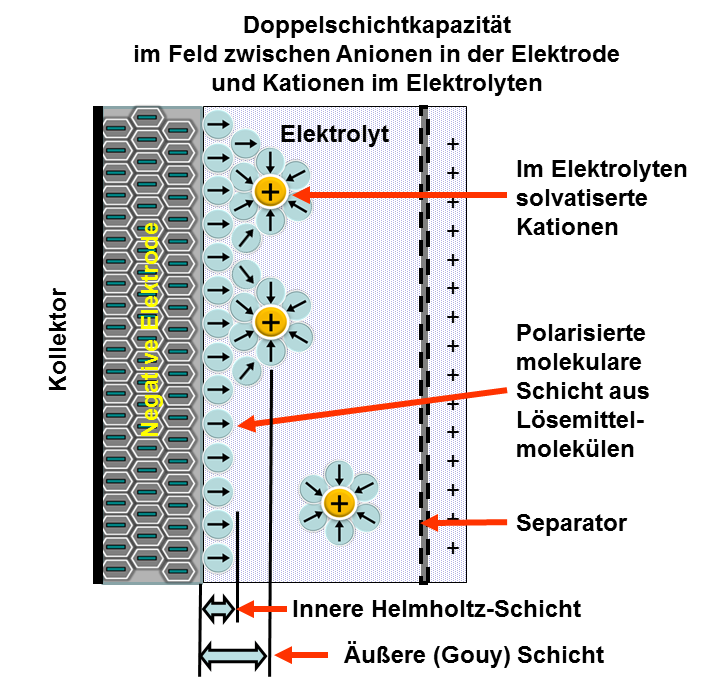
\includegraphics[width=0.5\textwidth]{Doppelschicht-Prinzipdarstellung}
	 \caption{Prinzipdarstellung der Doppelschichtkapazität. Quelle: Elcap (Own work) CC BY-SA 3.0, via Wikimedia Commons}
	 \label{abb_doppelschicht}
\end{figure}
In Shanghai werden Busse mit dieser Technologie seit 2008 im Linienverkehr eingesetzt, daneben werden Superkondensatoren für kurzzeitige Einsätze mit hohem Leistungsbedarf, zum Beispiel zur Bremsenergierückgewinnung oder zur Überbrückung stromloser Stellen in Trolleybussen eingesetzt \cite{Barminer-Busgesellschaft:2012}.
\subsection{Chemisch – Batterie}
\section{Vergleichstabelle}   %TODO: AUSFÜLLEN!
\begin{table}[htbp]\centering
	\begin{tabularx}{\linewidth}{XXX}
		\toprule
		A1 & B1 & C1 \\ \midrule
		A2 & B2 & C2 \\
		A3 & B3 & C3 \\ \bottomrule
	\end{tabularx}
	\caption{Übersicht Ladesysteme}
	\label{vergleichstabelle_speichertechnologien}
\end{table}
\chapter{Effizienzberechnung} %TODO: Besserer Titel %Drittens
\section{Ladesystem}
\section{Speichertechnologie}
\section{Ladestrategie und Route}
\section{Ergebnisse}
\subsection{Route A}
\subsection{Route B}
\chapter{Bewertung und Diskussion} %Diksussion
\section{Fazit}
\section{Ausblick}

%%%%% ENDE INHALT %%%%%

%Bibliographie
\bibliographystyle{alphadin}
\bibliography{Quellen/Quellenliste} 

\end{document}